\documentclass[11pt]{article}

\usepackage{a4wide}
\usepackage{xspace}
\usepackage[draft]{fixme}
\usepackage{amssymb}
\usepackage{amsmath}
\usepackage{graphicx}

\newtheorem{theorem}{Theorem}
\newtheorem{acknowledgement}[theorem]{Acknowledgement}
\newtheorem{algorithm}[theorem]{Algorithm}
\newtheorem{axiom}[theorem]{Axiom}
\newtheorem{case}[theorem]{Case}
\newtheorem{claim}[theorem]{Claim}
\newtheorem{conclusion}[theorem]{Conclusion}
\newtheorem{condition}[theorem]{Condition}
\newtheorem{conjecture}[theorem]{Conjecture}
\newtheorem{corollary}[theorem]{Corollary}
\newtheorem{criterion}[theorem]{Criterion}
\newtheorem{definition}[theorem]{Definition}
\newtheorem{example}[theorem]{Example}
\newtheorem{exercise}[theorem]{Exercise}
\newtheorem{lemma}[theorem]{Lemma}
\newtheorem{notation}[theorem]{Notation}
\newtheorem{problem}[theorem]{Problem}
\newtheorem{proposition}[theorem]{Proposition}
\newtheorem{remark}[theorem]{Remark}
\newtheorem{solution}[theorem]{Solution}
\newtheorem{summary}[theorem]{Summary}
\newenvironment{proof}[1][Proof]{\noindent\textbf{#1.} }{\ \rule{0.5em}{0.5em}}

\newcommand{\VAL}{\textsf{VAL}\xspace}
\newcommand{\CAL}{\textsf{CAL}\xspace}
\newcommand{\THEO}{\textsf{THEO}\xspace}
\newcommand{\ATOM}{\textsf{ATOM}\xspace}
\newcommand{\NOM}{\textsf{NOM}\xspace}
\newcommand{\FORM}{\textsf{FORM}\xspace}

\begin{document}

\title{Hybrid Type Theory\\ A Quartet in Four Movements}
\author{Carlos Areces \\
\and
Patrick Blackburn
\and
Antonia Huertas
\and 
Mara Manzano
}
\date{}
\maketitle

\begin{abstract}
This paper is about a logic\ldots and beauty. It tells the story of an idea that 
was born by putting together the work of four great names in in the history of 
Logic. 

The ideas of Reichenbach about the importance of temporal reference and
Prior about the importance of the internal perspective provided by modal and
tense logics have already been combined in~\cite{Blackburn1994}, In this
paper, simple hybrid logic, named propositional nominal tense logic, allowed
to put Reichenbach and Prior together. A decade later, in~\cite{ArecesBlackburn2005}, nominals were added to Montague's Intensional Logic to build
a richer hybrid logic (nominal intensional logic). The resulting system was
capable of capturing the insights of Reichenbach, Prior and Montague together.

What we shall do now is to add Leon Henkin's ideas of completeness proofs in
higher order systems to nominal intensional logic, which is presented here
as a hybrid type theory. Thus, this paper is about a very expressive formal
language, that is, type theory enhanced with hybrid modal resources. 
%Our
%collaboration with Carlos Areces and Patrick Blackburn grew 
%from~\cite{ArecesBlackburn2005}, producing the definition of a formal calculus for
%hybrid type theory and its completeness proof. 
As it is such a strong logic,
we looked towards Henkin's use of non-standard models in higher order logics
and we were able to adapt Henkin's general models thereby following in his
footsteps, and being loyal not only to his conception but also to the
construction Henkin proposed in his 1950 paper~\cite{Henkin1950}. Thus we
added Leon Henkin to the list of maestros that inspired this work.
We are sure Newton Da Costa will enjoy the quartet.
\end{abstract}

\begin{small}
\tableofcontents
\end{small}

%==========================================================================
\section{Introduction: The Quartet} \label{introduction}

\begin{center}
\begin{tabular}{cc}
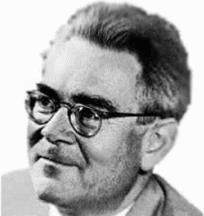
\includegraphics[scale=.5]{reichenbach_med.jpg} &
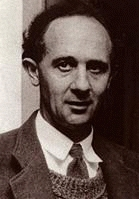
\includegraphics[scale=.6]{prior.jpg} \\
\emph{Hans Reichenbach}
& \emph{Arthur Prior}\\
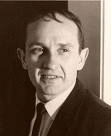
\includegraphics[scale=.8]{montague.jpg} &
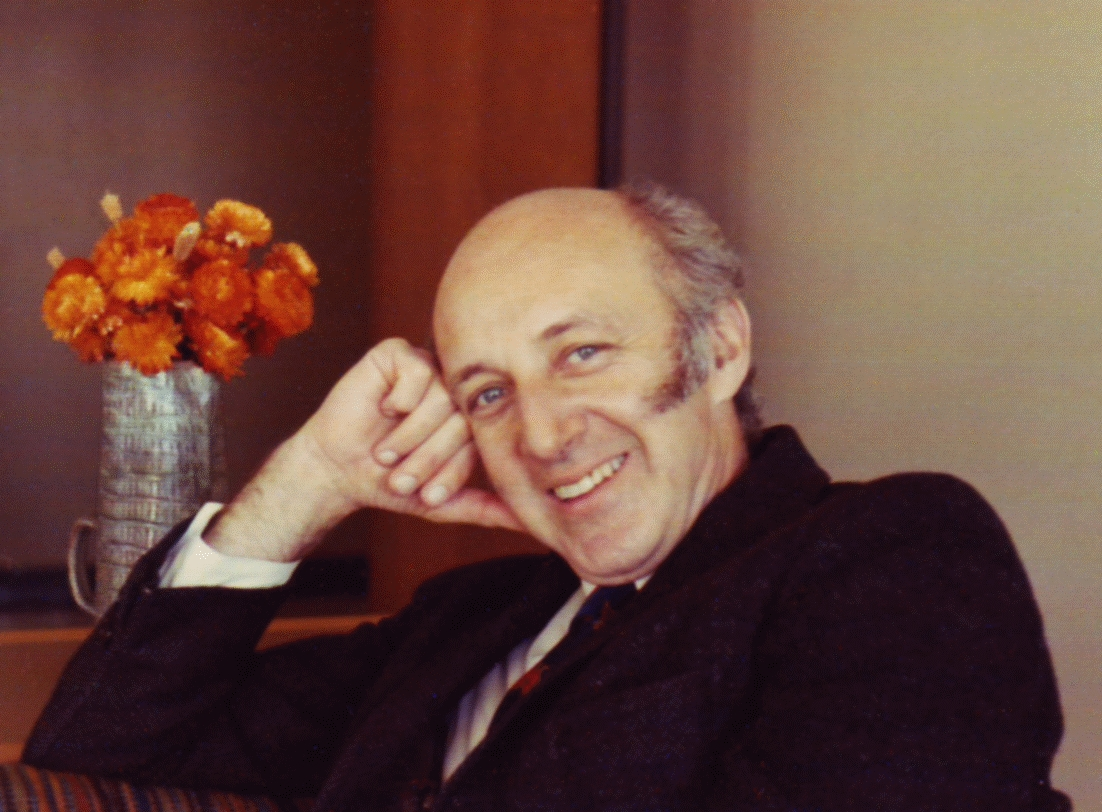
\includegraphics[scale=.1]{henkin73.jpg}\\
\emph{Richard Montague}
&\emph{Leon Henkin}
\end{tabular}%
\end{center}%

Hybrid type theory and its completeness proof will be presented in the next
sections.

Before this, in this introduction, a brief historical revision of the
important concepts that this article is about and of their four mentioned
inventors is presented.

\subsection{Reichenbach and tense referential analysis}

Hans Reichenbach in his book \emph{Elements of Symbolic 
Logic}~\cite{Reichenbach1947} included two chapters about the linguistic applications
of logic. It is especially relevant its treatment of tenses in natural
language. \emph{``Tenses determine time with reference to
the time point of the act of 
speech''}~\cite{Reichenbach1947} for him. He represented tenses in terms of reference with respect to
three temporal points: \emph{the point of speech} (S), \emph{the point
of event} (E), and \emph{the point of reference} (R). The point of speech
is the time at which the sentence is uttered; the point of event is the time
at which the event spoken of takes place. If we were to use only points S
and E, there are three possibilities for that point of event:
\emph{``before the point of speech''},
\emph{``simultaneous with the point of speech''}, 
and \emph{``after the point of speech''}. However, with these two kind of points only three
general tenses could be explained (past, present and future) and, as
Reichenbach pointed out, ``the number of verb tenses is
obviously greater''; in particular, there are tenses
concerning time order for two events. This is why he introduced \emph{the
point of reference}, a contextually determined time also present in tenses,
let us illustrate it with two examples.

When we say \emph{``Alba had sung''} there
is a clear intuition about some past time between 
\emph{the point of speech} and \emph{the point of event} when the singing event occurred. For
instance, we are telling our friends that we traveled to Barcelona to
attend Alba's concert but arrived too late, after Alba did sang. This
contextually determined past time is the point of reference. Accordingly,
the three dimensional representation of time ordering of the sentence 
\emph{``Alba had sung''} is E--R--S (where the
point of event is past the point of reference, which in turn is past the
point of speech). When we uttered \emph{``Alba
sang''}, we express that a singing event takes place at
some contextually determined past time, and its Reichenbach's tense
representation is E,R--S; that is, \emph{the point of event} and 
\emph{the point of reference} coincide and it is past the point of speech. In both
examples, the point of reference is some past time determined by the
context. In Figure~\ref{fig1} Reichenbach's representation of the English tenses by
using the three time markers is showed.

\begin{figure}[h]
\begin{center}
\begin{tabular}{|l|l|l|}
\hline
Structure & Name & \emph{Example} \\ \hline
E-R-S & Pluperfect & \emph{Alba had sung} \\ \hline
E,R-S & Past & \emph{Alba sang} \\ \hline
R-E-S or\ R-S,E or R-S-E & Future in the past & \emph{Alba would sing} \\ 
\hline
E-S,R & Perfect & \emph{Alba has sung} \\ \hline
S,R,E & Present & \emph{Alba sings} \\ \hline
S,R-E & Prospective & \emph{Alba is going to sing} \\ \hline
S-E-R or S,E-R or\ E-S-R & Future perfect & \emph{Alba will have sung} \\ 
\hline
S-R,E & Future & \emph{Alba will sing} \\ \hline
S-R-E & Future in the future & \textquestiondown ? \\ \hline
\end{tabular}%
\end{center}
\caption{Figure 1: Reichenbach's analyses of the tense forms of English.}\label{fig1}
\end{figure}

Reichenbach's analysis has had many objections; for instance, his use of
three different diagrams to represent the future in the past and the future
perfect tenses, or his little subtle analysis of the present perfect (simply
expressing that the point of reference corresponds to point of speech).
However, the \emph{point of reference} is a historically relevant
innovation. Without some way of expressing this kind of temporal reference,
many temporal constructions cannot be represented.

\subsection{Prior and tense logic}

Arthur Prior invented the orthodox tense logic, as a simple kind of modal
logic for reasoning about time. Prior introduced the internal perspective of
modal logics, where formulas are evaluated at some particular point within
models, as a way of capturing the \emph{``time-situated''} information. As the central
elements of his tense logic, he defined the $F$ and $P$ modalities (meaning 
\emph{``at some future time''}, and 
\emph{``at some past time''}, respectively). Let
us see how it works. Consider the present-tense English sentence 
\emph{``Alba sings''} and suppose that the
propositional symbol $\mathit{alba.sing}$ is its representation in tense logic. Now
consider the expression obtained by prefixing this with the $P$ operator, $%
P\ \mathit{alba.sing}$, which is true at a time $t$ if Alba does indeed sing at some
time $t_{0}$ before that $t$. However, this representation means that at
some completely unspecified past time Alba did sing, while the uttered
sentence \emph{``Alba Sang''} means that at some particular, contextually
determined, past time Alba did sing. Comparing with Reichenbach's analysis
Prior's representation captures only part of the meaning of the past-tense,
moreover it fails to capture the reference to specific times.

The \emph{time of speech} concept is fundamental to the internal
perspective and it fits perfectly with Prior's tense logic. It is simply the
particular time at which we evaluate a formula in a given model. It is also
fundamental the \emph{time of event} concept. In Prior's representation,
prefixing $\varphi $ to form $P\varphi $ or $F\varphi $ locates the point of
event to the past of \emph{the point of speech} or to the future of 
\emph{the point of speech}, respectively. Thus, Reichenbach's point of
speech and point of event are compatible with Prior's views of internal
perspective of tense logic. However, this is not the case for \emph{the
point of reference}. In the chapter 
\emph{``Precursors of tense-logic''} in his \emph{Past, Present and
Future}~\cite{Prior1967}, Prior dedicates a section to
Reichenbach's time of reference. Prior simply rejected Reichenbach's scheme
objecting among others that it did not cover new more complicated tenses as 
\emph{``I shall have been going to see John''}, where there are two points of references
(S-R2-E-R1) and then the point of speech could be seen as the 
\emph{first} point of reference. He also
explained his own solution: the systematic definition of complex tenses in
terms of simpler ones. The central concept of 
\emph{``presentness''} as the simplest tense is fundamental in this
systematic construction. Tensed utterances can be formed by using some
modifier to the \emph{``timeless propositional
context''}. Prior is thinking about some kind of idea of
\emph{``presentness''} as 
\emph{``timeless context''} and modifiers
operators dealing with past and future.

Prior's orthodox tense logic is very interesting and useful but it is not
able to capture the natural language tense nuances and the complexity of
real tense information.

\subsection{Montague and intensional logic}

Richard Montague thought that there is not an important theoretical
difference between natural languages and logical formal languages. Moreover.
In his \emph{``Universal 
Grammar''}~\cite{Montague1970}, he tried to develop a universal syntax and semantics that
acted as the framework for both types of languages. In his
\emph{``The Proper Treatment of Quantification in Ordinary
English''}~\cite{Montague1973}, Montague tried to present
syntax and semantics of a fragment of English rigorously. To do this, he
presented a logic system (where, in particular, rules of the tenses are
formalized) which he called \emph{Tense Intensional Logic}. He used Prior's 
$F$ and $P$ operators in that tensed variant of his Intensional Logic. There,
the central elements are types, used to capture the information on analysis
trees.

To interpret a linguistic expression is to assign intentions instead of
denotations, for him. An interpretation structure is of the kind 
$\langle \mathcal{A},I\rangle$ were $I$ is the \emph{set of
time moments} ($I$ is lineally ordered), where formulas can have different
denotations of truth values in different instants $i\in I$. Thus, for each 
$i\in I$, there would be a model $\langle \mathcal{A},i\rangle$.
Whereas the interpretation $\langle \mathcal{A},I\rangle $ assign
intentions (functions from $I$ in the truth values or denotation sets) to
each expression or formula. Montague's idea is to conceive tenses as acting
on the intentions of the formulas instead of acting on the 
extensions~\cite{Montague1973}; for instance, the truth value of a linguistic expression in
past tense, that is, its value in an instant $i$, depends on the values in
instants different from $i$.

\subsection{Henkin and the completeness of type theory}

Right at the introduction of his paper ``Completeness in the
theory of types''~\cite{Henkin1950}, Henkin recalls the
known facts on the completeness/incompleteness issue, at that moment:

\begin{itemize}
\item The completeness of the first order calculus (G\"{o}del 1930): 
\emph{``\ldots each formula of the calculus is a formal theorem which
becomes a true sentence under one of a certain intended class of
interpretation of the formal system.''}

\item The incompleteness of the second order calculus (G\"{o}del 1931): 
\emph{``\ldots no matter what (recursive) set of axioms are
chosen, the system will contain a formula which is valid but not a formal
theorem.''} To interpret the language we use standard models where
\emph{``\ldots the individual variables are interpreted as ranging over an (arbitrary)
domain of elements while the functional variables of degree n range over all
sets of ordered n-tuples of individuals.''}
\end{itemize}

Leon Henkin studied incompleteness problems of higher order systems, like
the already mentioned G\"{o}del's incompleteness problem. G\"{o}del had
shown how to construct logically valid sentences (in standard models)\ which
were no formal theorems of the second order calculus. The problem persists in
any possible calculus: \emph{``no matter what (recursive)
set of axioms are chosen\ldots valid but not a formal theorem''}.

In~\cite{Henkin1950}, he explained the key point to have
completeness in higher order systems: \emph{``\ldots there is a
wider class of models \ldots redefine the notion of a valid formula\ldots second
order calculus is complete: a formula is valid if and only if it is a formal
theorem''}.

How did Henkin prove in his doctoral dissertation, in 1947, the completeness
theorem for type theory?

A very quick answer to this question is: by changing the semantics and hence
the logic. Let's see the second order case. We have $\mathcal{SS}$, the class of standard structures, and accordingly, we find $\VAL_{\mathcal{SS}}$, the set of validities in the class. We know that there is
no complete calculus for $\VAL_{\mathcal{SS}}$, since this set is
not recursively enumerable. But even knowing that there is no calculus in
the standard sense, we have certain axioms and rules which are sound and so
we define a calculus $\CAL$.

Since the set $\THEO$ of logical theorems is a proper subset of 
$\VAL_{\mathcal{SS}}$ , in order to get the right semantics for it, we
need to widen the class of structures to reduce the set of validities (the
wider the class, the smaller the set, because to be valid in a wider class
of structures a sentence needs to pass more, shall we say, 
\emph{``quality controls''}). We are very
restricted when asking the relational universes of any model to contain all
possible relations ---\emph{i.e.}, structures where $A_{n}=\mathcal{\wp }%
A^{n}$, for all $n$--- If we also allow non-standard structures ---\emph{i.e.}, structures where $A_{n}\subseteq \mathcal{\wp }A^{n}$, for all $n$ , but
for some $m$, $A_{m}\neq \mathcal{\wp }A^{m}$--- then the set of validities
in the very large class of structures which includes both classes is
considerably reduced. Apart from being a subset of the power set of the 
$n$-ary cartesian product of the universe of individuals, if we do not impose
any other condition on the universes of a structure, it may well happen that
it fails to contain certain relations that are definable in the structure
using second order formulas: This means the comprehension schema does not
necessarily hold. That is why we need structures where the relational
universes obey certain closure conditions: \emph{Henkin's general models}.

With the semantics of general structures, completeness (in both weak and
strong senses), L\"{o}wenheim-Skolem and all these theorems can be proved as
in first order logic. In fact, he first proved the completeness of type
theory and later on found a way to apply a similar method for first order
logic.

In his ``The discovery of my completeness
proofs''~\cite{Henkin1996} Henkin explained the real
process for him to invent his \emph{``general
models''} to interpret the pure functional calculus of
second order. His idea was that G\"{o}del`s valid (in standard models) but
not provable sentences were very special; and that by simple redefining what
a valid formula is, these troubled formulas could not be valid anymore. The
proof of Henkin's completeness theorem for higher order logic gives a
general method for constructing such general models, and, in particular,
what is now more important for us, a detailed proof of completeness with
respect to general models is done for a logical system of infinite order in
the form of a theory of types.



%==========================================================================
\section{The Modal Scale}
\fixme{Start with an general introduction on modal logic}

\fixme{Then  switch to '\textbf{basic} modal logic}

The previous section was all about \emph{ideas}.  We have introduced
the different musical themes (and hinted to the way they relate to 
each other) that we will weave into our composition.  In this section 
we will start our formal work, by introducing the musical scale in 
which the composition will be cast: \emph{Modal Logic}.

The classical perspective on modal logic will tell that they are obtained 
from classical standard logic systems
---propositional logic, first-order logic, second order logic, etc.--- by
adding \emph{``non-truth-functional''}
operators, named modalities; the goal being to use these operators 
to gain the ability to \emph{qualify truth}.

Indeed, classicists would maintain that in modal Logic truth can be qualified. 
That is to say, beyond its descriptive or denotative content, expressions have 
also an auto-reflexive dimension. 
%Modal formalism are able to capture dynamic
%instances, in which truth can be relative. 
Some traditional qualifiers are: necessity, possibility, 
contingency, obligation, belief, knowledge, temporality, etc. In fact, 
if something is shown by this perspective, is that there
is not a unique modal logic but a whole family of them.

From a contemporary perspective, modal logics serve many purpuses.
To start with, and in complete accordance with the classical view, 
modal logics are recognized as marvelous tools for modeling and proving. 
Many notions in linguistic, philosophy, computing and science, etc.\ have a 
\emph{modal} character. Modal logic, thus,
provides a language and semantics to represent these notions in a rigorous
way. They also provide different reasoning mechanisms to obtain deductions or
derivations. Modal languages and their corresponding inference systems has been 
used to model and reason on situations involving \emph{necessity}
and \emph{possibility}, \emph{time}, \emph{beliefs}, \emph{computation}, and
many other. Crucially, all these applications share graph-like structures to represent
their main concepts (networks of possible worlds, flows of time, epistemic
alternatives, computational states, etc.)

More recently, modal logics have been recognized as tools for identifying interesting 
fragments of classical logics (via translation techniques)~\cite{Blackburnetal2007}. 
Modal logics can be seen as fragments of standard logics that inherit its standard semantics
(in terms of relational models) but with restricted expressive power. 
In this way, modal logics can be used to define logical subsystems of well know classical 
languages like first- or higher-order logics, but with specially tailored properties 
such as the decidability property of many modal logics. In
particular, under this view, modal logics are interesting tools to study the
balance between expressiveness and computational complexity in formal systems.

%\subsection{The relational semantics impact}
%
%The best known style of modal semantics is the \emph{relational} or 
%\emph{Kripke} semantics. After studying the class of Kripke models and their
%semantics, it is easy to reach the conclusion that pure modal logic axioms
%capture semantical properties of the accessibility relation $R$, \emph{i.e.},
%modal formulas are valid in models with the corresponding property of $R$:
%
%\begin{itemize}
%\item $T:=\square \varphi \rightarrow \varphi $ is valid, for reflexive $R$
%
%\item $4:=\square \varphi \rightarrow \square \square \varphi \ $ is valid,
%for transitive $R$
%
%\item $D:=\square \varphi \rightarrow \Diamond \varphi $ is valid, for
%serial $R$
%
%\item $B:=\varphi \rightarrow \square \Diamond \varphi $ is valid, for
%symmetric\ $R$
%
%\item $5:=\Diamond \varphi \rightarrow \square \Diamond \varphi $ is valid,
%for euclidean\ $R$
%
%\item $G:=\Diamond \square \varphi \rightarrow \square \Diamond \varphi $ is
%valid, for incestuous\ $R$
%\end{itemize}
%
%In fact, the axioms of a modal logic try to characterize the properties of
%their own accessibility relation. The language is very effective, but not
%always successful. Moreover, we have other alternatives languages. To put it
%succinctly:
%
%\begin{itemize}
%\item Modal models are relational structures and they are extremely common
%in \textit{Classical Model Theory}. 
%
%\item On the other hand, temporal relation is \emph{asymmetric} and
%\emph{irreflexive}, but these are not definable in orthodox tense logic.
%\end{itemize}

\paragraph{Evaluating modal logic}

Modal logics are a counterpart of classical logics. The question is what do
we gain when shifting from classical to modal logic? There are five key
points that make modal logics a very useful tool:

\begin{enumerate}
\item Better understanding, precision and useful axiomatization of the
structures formed by \emph{states, transitions} and \emph{procedures}.

\item Very concise formal expression (operator designated \emph{ad hoc})

\item Modal logics are \emph{decidable}, which is an improved situation in
comparison to the one encountered in FOL or other higher order logics.

\item \emph{Locally} focused: to better understand the \emph{structure of
transitions} between states we place ourselves inside the structure and
travel along

\item We gain an \emph{internal }perspective (AUTOMATON:= visiting the
accessible states)
\end{enumerate}

On the other hand, what is missing when shifting to modal logics?

\begin{enumerate}
\item States are crucial, but we cannot refer to them.

\item The accessibility relation is essential, but it is not explicit in the
language.

\item In tableau calculus metalanguage tools are needed to solve this
shortcoming.
\end{enumerate}

%==========================================================================
%\subsection{Hybrid logic}

\subsection{A Hybrid Melody}

\fixme{relate this to ``point of reference''} Prior~\cite{Prior1967} objected Reichenbach's ideas about the point of
reference. This is ironic, as Areces and Blackburn pointed 
out~\cite{ArecesBlackburn2005} since in that same book~\cite{Prior1967}, Prior introduced
a tool that allows integrating his own ideas with those of Reichenbach in a
very simple way.

This tool's key idea is to add a second sort of propositional symbols ($i$, $%
j$, $k$, etc.), called nominals, to the propositional symbols of orthodox
tense logic ($p$, $q$, $r$, etc.). Nominals allow to formally ``talk'' about
time instants because each nominal symbol is only true at exactly one time in any
model; the time the nominal \emph{``is naming''}. Nominals will be the central
element of \emph{modern hybrid logic}. This is a simple change, but it
immediately produces a more expressive logic, named here \emph{nominal tense
logic}~\cite{Blackburn1994}. Let's see what this means.

Consider the formula of orthodox tense logic
$$
F(r\wedge p)\wedge \ F(r\wedge q)\rightarrow F(p\wedge q)
$$
expressing that if in the future there is a time where both $r$ and $p$ are
true together, and in the future there is a time where $r$ and $q$ are true
together, then there is a time in the future where $p$ and $q$ are true
together. It is clearly not always true because the future times that
witness $p$ and $q$ could be different. Now consider the formula of nominal
tense logic obtained by replacing the propositional symbol $r$ by the nominal
symbol $i$ 
$$
F(i\wedge p)\wedge F(i\wedge q)\rightarrow F(p\wedge q)
$$
This formula is true in every model because the future times witnessing $p$
and witnessing $q$ are both making the nominal $i$ true, and there is only
one time doing this for $i$, by definition. Thus, there is a future time
where $p$ and $q$ are both true, something expressible in nominal tense
logic.

Therefore, nominals allow to express Reichenbach's
points of reference. Moreover, representations in nominal tense improve
Reichenbach's representations~\cite{ArecesBlackburn2005}. As an example,
consider the formula $P(i\wedge P\varphi )$ stating that there is some time
in the past, named with the nominal $i$, and that the event $\varphi $
happened before that past time. It is the representation of the pluperfect
modelization of Reichenbach and combines Reichenbach's insight on the role
played by temporal reference with Prior's insistence on the privileged role
of tensed talk. Figure~\ref{fig2} shows a modification of the table given earlier,
obtained by adding nominal for tense logical representations. In some cases
the nominal tense logical representations improve Reichenbach's. For
instance, the future-in-the-past now has a single representation: the
formula $P(i\wedge F\varphi )$ expresses that there is a reference time $i$
in the past, and that the point of event occurs to the future of $i$, which
is what the future-in-the-past means. With this representation, it is not
necessary to use irrelevant different positions of the point of reference
with respect to the point of speech, as Reichenbach did.

\begin{figure}[h]
\begin{center}
\begin{tabular}{|l|l|l|}
\hline
\textbf{Structure} & Representation & \emph{Example} \\ \hline
\textbf{E-R-S} & $\left\langle P\right\rangle (i\wedge \left\langle
P\right\rangle \varphi )$ & \emph{Alba had sang} \\ \hline
\textbf{E,R-S} & $\left\langle P\right\rangle (i\wedge \varphi )$ & \emph{%
Alba sang} \\ \hline
\textbf{R-E-S }or\textbf{\ R-S,E }or \textbf{R-S-E} & $\left\langle
P\right\rangle (i\wedge \left\langle F\right\rangle \varphi )$ & \emph{%
Alba would sing} \\ \hline
\textbf{E-S,R} & $i\wedge \left\langle P\right\rangle \varphi $ & \emph{%
Alba has sung} \\ \hline
\textbf{S,R,E} & $i\wedge \varphi $ & \emph{Alba sings} \\ \hline
\textbf{S,R-E} & $i\wedge \left\langle F\right\rangle \varphi $ & \emph{%
Alba is going to sing} \\ \hline
\textbf{S-E-R} or \textbf{S,E-R }or\textbf{\ E-S-R} & $\left\langle
F\right\rangle (i\wedge \left\langle P\right\rangle \varphi )$ & \emph{%
Alba will have sung} \\ \hline
\textbf{S-R,E} & $\left\langle F\right\rangle (i\wedge \varphi )$ & \emph{%
Alba will sing} \\ \hline
\textbf{S-R-E} & $\left\langle F\right\rangle (i\wedge \left\langle
F\right\rangle \varphi )$ & \textquestiondown ? \\ \hline
\end{tabular}%
\end{center}

\caption{Reichenbach`s referential analysis of tense using nominals}\label{fig2}
\end{figure}

In nominal tense logic we can find the following characteristic elements of
hybrid modern logic:

\begin{itemize}
\item \textbf{Nominals}. Prior invented a representation for referring to
instants of time: \emph{sorting the propositional symbols and using terms
as formulas} 
$$
\ATOM \cup \NOM
$$
The atomic formulas $i\in \NOM$ received the expected
interpretation, just a singleton.

\item \textbf{Universal modality}. The diamond form of the universal
modality is $\mathbf{E}$\fixme{not mentioned before}

\item \textbf{Quantifiers}. Prior added the quantifiers $\forall$ and 
$\exists$ allowing then to bind nominals
\end{itemize}

This is neat. However, as we pointed out at the start of the paper, the
discussion has been conducted within the confines of propositional nominal
tense logic. If we want to apply these ideas to real grammars for natural
language, that is not good enough. And this leads us to the main topic of
the paper: adding nominals to Montague's IL.

\subsection{Counterpoint}

\emph{States} are crucial in modal semantics but we cannot refer to them with the formal logic. But we can in hybrid logic!. In fact in hybrid logic
we enhance expressivity of modal logic:

\begin{itemize}
\item To introduce explicit references to the elements of the model domain;
for instance, states, days, years, etc.

\item To express that two elements of the domain are related; \emph{i.e.,}
a moment precedes another

\item To improve expressive power by modeling time indexicals; as an
example, yesterday, today, tomorrow, now, etc.

\item To have an elegant proof theory, closed to labelled deduction systems

\item To define properties of frames which are relevant to temporal logic
(irreflexivity, asymmetry)
\end{itemize}

Hybrid logic builds on modal simplicity whilst adding nominals and the $@$
operator to improve its expressive power. 
Nominals refer to individual nodes in the Kripke structure and the $@$
operator allows us to state in the object language that a formula is true at
a given point, while the accessibility relation becomes explicit.

As already noted, in a hybrid language we have two sorts of atomic formulas;
namely $\ATOM \cup \NOM$. We add a new set of modal
operators $\{ @_{i}\mid i\in \NOM\}$ and we form new
formulas in this extended language: $\NOM \subseteq \FORM$ FF
and $@_{i}\varphi \in \FORM$.

In the hybrid semantic we still have Kripke models and we add interpretation
of new formulas:
$$
\mathcal{A},w\Vdash i~\ \text{iff\ }~\text{the instant }w\text{ is named\ }i%
\text{ iff \ }i^{\mathcal{A}}=\left\{ w\right\}
$$
while the interpretation of the new operator $@$ reads%
$$
\mathcal{A},w\Vdash @_{i}\varphi ~\ \text{iff\ }~\mathcal{A},v\Vdash \varphi
$$
$v$ being the unique element of $W$ where $i$ is true, namely 
$i^{\mathcal{A}}=\{v\}$.

\emph{Reflexivity}, \emph{symmetry} and \emph{transitivity} of identity are
now \fixme{pure formulas not introduced before} pure formulas:%
$$
@_{i}i\qquad @_{i}j\rightarrow @_{j}i\qquad @_{i}j\wedge @_{j}k\rightarrow
@_{i}k
$$
And we can also express that two points are accessible: $@_{s}\Diamond t\ $%
says that states named by $s\ $and\ $t$ are related by accessibility\ $R$

\emph{Reflexivity}, \emph{symmetry} and \emph{transitivity} of accessibility
are pure formulas as well:%
$$
@_{i}\Diamond i\qquad @_{i}\square \Diamond i\qquad \Diamond \Diamond
i\rightarrow \Diamond i
$$

\emph{Irreflexivity}, \emph{asymmetry}, \emph{antisymmetry} and\emph{\
intransitivity} of accessibility are also pure formulas: 
$$
@_{i}\lnot \Diamond i\qquad @_{i}\lnot \Diamond \Diamond i\qquad
@_{i}\square (\Diamond i\rightarrow i)\qquad \Diamond \Diamond i\rightarrow
\lnot \Diamond i
$$


\paragraph{Zen Philosophy.}
As an example of the expressive power of hybrid logic let us see the
following.

In \emph{The book of perfect emptiness} Tang de Ying asked Xia Ge: 
\emph{``Did things exist at the dawn of time?''}.

Xia Ge answered: \emph{``If things had not existed at the
dawn of time, how could they possibly exist today? By the same token, men in
the future could believe that things did not exist today.''}

This argument can be reformulated in this way.

\begin{itemize}
\item $\alpha :=\;$\emph{If things exist at a given point in time, then at
any given previous moment in time things must have existed.}

\item $\beta :=\;$\emph{Things exist today.}

\item $\gamma :=\;$\emph{The dawn of time is previous to all else.}

\item $\delta :=\;$\emph{Things existed at the dawn of time.}
\end{itemize}

In hybrid temporal logic we can express this argument quite simply:

Hypothesis:

\begin{itemize}
\item $\alpha := q \rightarrow [P]q$

\item $\beta := @_hq$

\item $\gamma := @_a[P]\perp$
\end{itemize}

Conclusion

\begin{itemize}
\item $\delta := @_a q$
\end{itemize}

To prove $\delta$ from the hypothesis we can use the trichotomy axiom of
temporal logic 
$$
@_a h\vee @_a \langle P\rangle h \vee @_h \langle P\rangle a
$$


%==========================================================================
\section{Hybrid type theory}

\subsection{Montague grammar and nominal intensional logic}

The following definitions follow Montague's treatment; the only deviations
from his original work are the clauses we have added for handling nominals
and the introduction of the $@$ operator...

As usual the set $\mathsf{TYPES}$ is defined recursively 
\begin{equation*}
\mathsf{TYPES}::=t\mid e\mid \langle a,b\rangle
\end{equation*}

The set $\mathsf{ME}_{a}$ of meaningful expressions of type\textbf{\ }$a$ is
defined recursively as follows:

\begin{enumerate}
\item Every nominal $i$ is in $\mathsf{ME}_{t}$

\item Every constant of type $a$ is in $\mathsf{ME}_{a}$, for any type $a$

\item Every variable of type $a$ is in $\mathsf{ME}_{a}$, for any type $a$

\item If $\alpha \in \mathsf{ME}_{a}$ and $u_{b}$ is a variable of type $b$,
then $\lambda u_{b}\alpha \in \mathsf{ME}_{\langle b,a\rangle }$

\item If $\gamma \in \mathsf{ME}_{\langle b,a\rangle }$ and $\beta \in 
\mathsf{ME}_{b}$ then $\gamma \beta \in \mathsf{ME}_{a}$

\item If $\alpha $ and $\beta $ are both in $\mathsf{ME}_{a}$, then $\alpha
=\beta \in \mathsf{ME}_{t}$

\item If $\varphi $ is in $\mathsf{ME}_{t}$, then $\lnot \varphi $ is also
in $\mathsf{ME}_{t}$

\item If $\varphi $ and $\psi $ are in $\mathsf{ME}_{t}\ $, then $\varphi
\wedge \psi $ is in $\mathsf{ME}_{t}$

\item If $\varphi $ is in $\mathsf{ME}_{t}$ and $u_{a}$ is a variable of any
type $a$, then $\exists u_{a}\varphi $ $\ $is in $\mathsf{ME}_{t}$\textbf{\ }

\item If $\varphi $ is in $\mathsf{ME}_{t}$, then $\Diamond \varphi $ is in $%
\mathsf{ME}_{t}$

\item If $\alpha $ is in $\mathsf{ME}_{a}$, then $@_{i}\alpha \in \mathsf{ME}%
_{a}$
\end{enumerate}

\subsection{Semantics}

The structures used to interpret this powerful language contain a hierarchy
of types plus the usual ingredients of Kripke's structures; namely, a
universe of worlds and the accessibility relation. We also have a function
giving to each constant in the language its appropriate interpretation in the
hierarchy.

A (standard) structure for $\mathcal{HTT}$ is a pair 
$\mathcal{M}=\langle \mathcal{S},\mathsf{F}\rangle $ such that%
$$
\mathcal{S}=\left\langle \langle \mathsf{D}_{a}\rangle _{a\in \mathsf{TYPES}%
},W,R\right\rangle
$$
is a skeleton, where:

\begin{enumerate}
\item $\langle \mathsf{D}_{a}\rangle _{a\in \mathsf{TYPES}}$, the hierarchy
of types, is defined recursively as follows (where $a$ and $b$ are types):%
$$
\begin{array}{rcl}
\mathsf{D}_{e} & = & A\text{ (where }A\not=\varnothing \text{ is the set of
individuals)} \\ 
\mathsf{D}_{t} & = & \text{ is a two element set (the truth values)} \\ 
\mathsf{D}_{\langle a,b\rangle } & = & \mathsf{D}_{b}{}^{\mathsf{D}_{a}}%
\text{ is the set of all functions from }\mathsf{D}_{a}\text{ into }\mathsf{D%
}_{b}%
\end{array}%
$$

\item $W$ is the set of worlds, $W\not=\varnothing $

\item $\mathsf{R}\subseteq \mathsf{W}\times \mathsf{W}$ is the accessibility
relation

\item $\mathsf{F}$ is a function whose domain is $\mathsf{NOM}\cup \mathsf{%
CON}$ of $\mathcal{HTT}$, $\mathsf{F}$ assigns to each nominal a function
from $\mathsf{W}$ to the set of truth values and to each non-logical
constant a function from $\mathsf{W}$ to an element in the hierarchy of
types of the appropriate type 
\begin{equation*}
\mathsf{F}:\mathsf{NOM}\cup \mathsf{CON}\longrightarrow \bigcup\limits_{a\in 
\mathsf{TYPES}}\left( \left. \mathsf{D}_{a}\right. ^{W}\right)
\end{equation*}
\end{enumerate}

%==========================================================================
\section{Conclusions}\label{conclusions}

XXX


\bibliographystyle{plain} 
\bibliography{dacosta10}

\end{document}
